\documentclass[man]{apa2}
\usepackage{pslatex}
\usepackage{amssymb}
\usepackage{graphicx}
\usepackage{color}
\usepackage{covington}
\usepackage[usenames,dvipsnames]{xcolor}

\title{
%Pragmatic contrast helps preschoolers learn category structure\\
%Pragmatic inferences as a route to learning category structure\\
%Learning about the world through pragmatic inference
Children's pragmatic inferences as a route for learning about the world}
%Developing the ability to learn about the world through pragmatic inference
%Pragmatic inference can help children learn about the world}

\twoauthors{Alexandra C. Horowitz}{Michael C. Frank}
\twoaffiliations{Department of Psychology, Stanford University}{Department of Psychology, Stanford University}


\abstract{Information about the world is not always stated explicitly. We investigated whether children can infer generalizable information pragmatically from speakers' word choices. We introduced novel objects described with prenominal adjectives and asked what other category members look like. Preschoolers from a university nursery school and local children's museum reliably inferred implied contrast with the support of framing cues (Experiment 1).  Performance was reduced after removing the contrastive framing, but improved after a pre-exposure to the relevant adjective pairs (Experiment 2). In a free-response task, children spontaneously produced relevant property contrasts (Experiment 3). Contrast inferences did not differ  even when the polarity of the adjectives was reversed (Experiment 4). Our findings suggest that preschoolers generalize from a single exemplar--- not just about what that category is, but also what it isn't. Sensitivity to the implications of speakers' production choices may help children learn about the world. 


%Children learn many facts through direct instruction (e.g. ``red lights mean stop''), but not all knowledge is stated explicitly.  We investigate the hypothesis that children infer generalizable information about the world pragmatically by making inferences from speakers' word choices. We described novel objects to preschoolers using a prenominal adjective (e.g. ``this is a [small/broken] tibu''). We then asked what they thought members of the object's category typically looked like (e.g. bigger or unbroken).  In Experiment 1, we used a supportive contrastive framing and found that children reliably inferred that typical category members differed on the property used in the description.  In Experiment 2, children's performance was reduced when the contrastive framing was removed, but improved after a pre-exposure to the relevant adjective pairs. In Experiment 3, a free-response task, children spontaneously produced relevant property contrasts.  Our findings suggest that preschoolers can learn about a novel category from a single exemplar--- not just about what that category is, but also what it isn't. More generally, sensitivity to the implications of speakers' production choices may allow children to learn efficiently about the world.


~\\

Keywords: pragmatics; language development; adjectives; knowledge transmission}

\shorttitle{Learning through pragmatics}
\rightheader{Learning through pragmatics}

\acknowledgements{Special thanks to the staff and families at the Bing Nursery School and the Children's Discovery Museum of San Jose and to Octavia Zahrt for assistance with Experiment 3. This work supported by a John Merck Scholars Fellowship and ONR grant N00014-13-1-0287. Earlier versions of this work were presented to the Cognitive Science Society in \citeA{horowitz2012} and \citeA{horowitz2014}.

~\\

\noindent Address all correspondence to Alexandra C. Horowitz, Stanford University, Department of Psychology, Jordan Hall, 450 Serra Mall (Bldg. 420), Stanford, CA, 94305. Phone: 650-721-9270. E-mail: \texttt{ahorowit@stanford.edu}}

\begin{document}

\maketitle                            


\section{Introduction}

Children learn much important information through explicit instruction (e.g., ``put the fork on the left of the plate'') and generic statements (``forks go on the left''), but not all information is stated directly. Sometimes information is implicit in the particular production choices a speaker makes. For example, if a parent says, ``that's a salad fork,'' she is implicitly conveying that forks vary in the foods they are intended for (and that most other forks are likely used for non-salad items). More generally, the way we describe the world can reveal to a perceptive observer all sorts of biases about what we find notable, interesting, or generally worthy of comment---and such biases can in turn act as signals about our knowledge of the world. Are children able to use these implicit signals for learning? 

We address this question using a simple case study: learning to generalize novel words via minimal contrastive descriptions.  We focus on contrastive word choices, as in the above ``salad fork'' example. Contrastive word choices---the way we use labels and their modifiers---can help identify the speaker's intended referent in the current context (selecting the desired fork) but can also jointly signal generalizable knowledge (forks are associated with meal courses). In the current study, we investigate the idea that adults and children may learn generalizable knowledge via inferences about why speakers choose a particular word to convey a message. To motivate this case study, we begin by discussing two bodies of research: first, work on children's ability to learn about the world from language, and second, work on their ability to reason about the knowledge and beliefs underlying other agents' actions (both non-linguistic and linguistic). 

% This work motivates our current studies: Three experiments investigating preschoolers' generalizations about unseen category members based on speakers' word choices. 

\subsection{Learning from others' explicit statements}

Although learning from the world directly is a very powerful method for acquiring knowledge \cite{gopnik2012b}, there is no way that even the most precocious child-scientist could reconstruct an adult's knowledge from direct experience alone \cite{shafto2012,harris2012}. Instead, children's knowledge comes from a mixture of direct experiences and knowledge transmitted by others. 

Language is an extremely powerful source of cues about the world. From the time children begin to speak, they understand that language is used to communicate information \cite{vouloumanos2012,martin2012}. They expect speakers of the same language to use conventional names for conventional meanings \cite{clark1987, markman1988, diesendruck2005}, but learn to recognize that individual knowledge such as facts about objects may not be shared \cite{diesendruck2001}. They also show early knowledge that language can share information that goes beyond the here-and-now \cite{saylor2007,ganea2007}. This early, foundational set of assumptions---that speakers use language in consistent and communicative ways to convey (relatively) abstract knowledge---is critical in allowing children to use language to learn about the world. 

While some language describes the current state of the world (e.g., ``the salad fork is on the outside''), other statements provide more general information that applies across situations (``salad forks go on the outside''). Generic language---cued in a number of ways, including the use of a bare plural (e.g. ``salad forks'')---is a particularly powerful method for conveying such information \cite{leslie2008}. Children can use generic language to infer general properties quite early \cite{gelman2003}. They draw different conclusions from generic statements than non-generic statements, and are more likely to believe that information stated generically is  conceptually and functionally central and more widely-known \cite{cimpian2009, cimpian2010, cimpian2012}. And in some contexts, generic language is not even necessary: The simple use of a label or even the use of particular communicative cues---child-directed speech, direct gaze, or pointing---may signal that a speaker is presenting information that is relevant to a kind, category, or practice \cite{csibra2009, butler2012}. 
% One striking example of the role of labeling comes from a study in which \citeA{rakoczy2008} introduced 2- and 3-year-old children to a game featuring an action called ``daxing.'' Children then saw a character perform a different action and label it daxing or not.  Both age groups were more likely to protest the new action when it violated their expectations about the meaning of daxing than when it was unlabeled. By age 3 children were more likely to provide explicitly normative protests (e.g. ``It doesn't go like that'') than imperative protests (e.g. ``Use the stick''). Providing a label for the action led children to expect and enforce that the action was specific and inflexible to other interpretations.  

Language is such a powerful source of information that preschoolers find it very difficult \emph{not} to believe what they are told.  Three-year-olds can discount inconsistent evidence conveyed through physical markers (e.g. they can learn that an agent purposely places a sticker on the wrong cup, and select the opposite), but they have a much harder time discounting verbal evidence from an unreliable speaker in the same scenario: Even after learning that the agent consistently states the \emph{wrong} location, children still look for the hidden item where the speaker says \cite{jaswal2010}.  When given the option to choose between two potential informants, however, preschoolers can recognize which speaker is more accurate and prefer to trust that speaker \cite{pasquini2007}, retaining this preference even after a time delay \cite{corriveau2009}.  In sum, children favor more reliable speakers when a choice is available, but they display a general bias to trust verbal information.





% To summarize: Explicit linguistic transmission is a powerful and important source of general information about both the specific and the abstract. From an early age children are able to make use of this information, recognizing a number of different cues to the generalizability of the information in a particular statement. We next turn to work on children's ability to make inferences about the unseen causes of actions, both linguistic and non-linguistic.


\subsection{Inferences about others' actions}

% Our work is based on the idea that children make rational inferences about peopleÕs actions.  

In nearly all of the work reviewed above, a parent, teacher, or experimenter presents the relevant information explicitly, via a demonstration or explicit utterance. But a parallel line of work suggests that children and even infants are able to make inferences about the \emph{implicit} sources of both linguistic and non-linguistic actions. This literature is critical for motivating our hypothesis---that such inferences might not just inform guesses about particular agents' knowledge, abilities, preferences, or desires, but that they might also be a source of information about the world more generally. 

% We begin by discussing work on non-linguistic actions and then move on to linguistic (pragmatic) inferences.

% \subsubsection{Inferences about others' non-linguistic actions}

By their first birthday, babies appear to make inferences about the unseen goals that underlie actions, even in very stripped-down displays.  For example, they look longer when a shape that previously jumped over a wall toward another shape continues on the same path when the wall is removed (an action goal) instead of moving directly toward the shape (an end-state goal; \citeNP{gergely1995}). This result is part of a broader body of work suggesting that infants expect agents to act rationally to achieve (inferred) outcomes most efficiently \cite{csibra1998, gergely2003}. In other words, very young children appear sensitive not only to agents' particular actions, but also to the presumed purpose for these actions. 

Young children also seem to be able to integrate information about constraints on knowledge and action into their inferences about goals. For example, infants can distinguish between actions that are produced intentionally (e.g. the choice of a particular ball by an agent viewing the contents of a box) versus randomly (by an agent wearing a blindfold; \citeNP{xu2009}).  They can also reevaluate the likelihood of particular evidence when physical constraints make it more difficult for certain items to be selected (e.g., balls that stick to velcro, \citeNP{denison2010b}).  They can even infer that an agent demonstrates a preference by observing a pattern of choices that would be unlikely to occur by random selection \cite{kushnir2010}. 

Critical for our hypothesis here, some evidence suggests that young children can also work backwards from agents' actions to infer generalizable knowledge about objects. In an experiment by \citeA{gweon2010}, fifteen-month-olds watched an experimenter pull a series of blue balls from a box and squeeze each toy to produce a squeaking sound. Babies were then handed a slightly different, yellow ball, and their generalizations about whether the new ball should also squeak were measured by their attempts to squeeze the toy. Depending on the evidence they saw, babies made different generalizations: If the blue balls were sampled by the experimenter from a box of mostly blue balls (implying that they were randomly sampled by the agent), they were more likely to think that a yellow ball would also squeak. But if they saw the blue balls picked out from a box of mostly yellow balls (where presumably the blue balls were less likely to be picked randomly, and thus were more likely to be intentionally selected for the demonstration of squeaking), they thought the yellow balls were less likely to squeak. In other words, children in this second condition made a general inference about the world (yellow balls don't squeak) based on a surprising thing that someone \emph{didn't} do (did not pick out more common, yellow balls). The experiments we present below test a related type of inference in the linguistic domain; we therefore describe some of the background for these kinds of pragmatic inference. 

% The inferences described above show a striking similarity to a quite different kind of inference: pragmatic inferences in language comprehension 

Similar to the patterns of reasoning described above, listeners make pragmatic inferences in language comprehension by reasoning about the generating causes of a speaker's (linguistic) action and about the constraints on that action \cite{shafto2012}. Just as babies form expectations about sampling likelihoods and infer that violations are intentional and informative (e.g. indicating others' preference or pedagogical demonstrations), they may learn to do the same for language, and make inferences about implicit, intended meaning when speakers' production choices differ from their expectations. Grice's \citeyear{grice1975} maxims of cooperative communication---be truthful, informative, relevant, and clear---provide a framework for inferring implied meaning from linguistic evidence. For instance, Grice gives an example of a recommender who declares that his student has good penmanship. This recommender is choosing an action that completes his goal---write a letter that is maximally informative about the student---while complying with the restrictions on his actions---be truthful, don't say anything negative. On the basis of the above letter of recommendation, a reader of the letter can make the \emph{implicature} that the writer does not believe the applicant has any other positive qualities (or else he would have mentioned them). A number of other theories have also attempted to describe the interplay between intention and production \cite{horn1984,clark1996,levinson2000}, all preserving the basic idea of pragmatic inference as action understanding. 

% In our current work, we take the simple case of modified referents to examine whether listeners infer that the decision to include an optional grammatical marker (the adjective) pragmatically conveys a speaker's intention to mark a relevant contrast dimension.
%Since we are interested here in whether children can learn based on pragmatic inferences, we briefly review work on children's general pragmatic abilities. Initial work in this domain suggested that children might show deficits in pragmatic language understanding through age five or even later \cite{noveck2000,papafragou2003}. When presented with a situation where three of three horses jumped a fence, children judged the utterance ``some of the horses jumped over the fence'' to be a felicitous description. While adults reject the statement under the assumption that ``some'' implies \emph{some but not all}, children accept that ``some'' can overlap in meaning with ``all''.  A more recent body of work, however, suggests that these deficits are specific to particular linguistic phenomena, namely scalar implicatures using quantifiers like ``some'' and ``all'' \cite{barner2011,katsos2011}.

%One interpretation of failures in scalar implicature tasks is that children have trouble holding in mind and contrasting the alternative statements ``some'' and ``all.'' This \emph{alternatives hypothesis} makes a number of predictions that have now been tested. First, children have difficulties with even non-pragmatic interpretations that require considering these alternatives (e.g., reasoning about what ``only some'' means; \citeNP{chierchia2001, barner2011}). Second, exposure to alternatives increases their success in computing implicatures \cite{skordos2014}. Third, they perform better in contexts where alternative meanings are more explicit (e.g. pictured as alternatives in a forced-choice) \cite{miller2005,stiller2014}. Thus, children appear to be more pragmatically sophisticated than the original results suggested. We appeal to the alternatives hypothesis below in describing the developmental pattern we observe in our experiments. 

\subsection{Our current study}

Given that children are able to make sophisticated inferences about the basis for both actions and utterances, we ask whether pragmatic inferences can provide a method for the transmission of information. In particular, we investigate preschoolers' ability to infer information about a general class from the specific word choices that a speaker makes in a description. For example, labeling a novel item as a ``tall blicket'' conveys not only that this item is a tall blicket, but also suggests that height is a relevant variable property to blickets. Therefore, other blickets may be short. 

We focus on adjectives as a case study.  Because adjectives are optional modifiers, they can selectively be included in an utterance to draw contrasts between an intended referent and other unintended alternatives. 
% Therefore, working backwards, if the listener does not know what the unintended alternatives are, the inclusion of an adjective could convey important information about contrasts that are relevant for a particular category or comparison. In this way, an optional modifier could provide important general information about what a specific case is being contrasted with.
Children show evidence of recognizing implied contrasts from prenominal adjectives (e.g. ``red car'') in their real-time language comprehension by age 3 \cite{fernald2010}, and in more complex visual contexts by kindergarten \cite{nadig2002}. Work to date has focused on how adjectives are used to identify targets in referential communication tasks, however.  Here we examine a novel question, asking how adjective use can help listeners infer \emph{what the context is} that would lead a speaker to produce a partiular modified description.  In other words, we ask whether children can infer that a contrastive description conveys not only information about the current referent, but also information about the implied property variability of other category members.

In the three experiments below, we test this hypothesis. In Experiment 1, we found that with a supportive framing, preschoolers made robust contrast inferences.  In Experiment 2, performance decreased in a more stripped-down version of the task with reduced cues to contrast but was somewhat increased by pre-exposure to the appropriate alternative set, supporting a pragmatic interpretation of this behavior. In Experiment 3, children succeeded in a more open-ended production task, suggesting that they were able to summon to mind the relevant contrast dimension and not just select between alternatives. In Experiment 4, contrast selections remained above chance regardless of the polarity of the adjective referenced.

\section{Experiment 1}

To investigate preschoolers' inferences about adjective use and category membership, we used a simple triad task.  We introduced children to a novel shape, followed by two similar shapes: one that differed from the first only by size (e.g. small versus big), and the other that differed from the first only by a different polar feature (e.g. wet versus dry).\footnote{In discussions of adjective semantics, the size adjectives we used are referred to as \emph{gradable} adjectives because their meaning is relative to the head noun \cite{kennedy2012}---a small sofa is nevertheless bigger than a large mouse. In contrast, our alternative features were \emph{non-gradable}---a sofa or a mouse exposed to water is equally considered wet. For convenience here and below, we refer to this distinction as ``size'' vs. ``feature.''} We described the first shape with either a size or feature adjective, and asked children to generalize what they thought other category members looked like. Children could follow at least two plausible strategies in this scenario. First, they could generalize from the exact property they heard, reasoning as follows: \emph{You said, `This is a special kind of tibu. This is a small tibu,' so most tibus are probably also small}. Second, they could generalize from the property \emph{dimension} they heard, reasoning instead that: \emph{You said, `This is a special kind of tibu. This is a small tibu.' If most tibus were small, you probably wouldn't have pointed out this one's size as special. So other tibus probably vary by size and can be big.} If children are sensitive to the pragmatic implications of speakers' choices, then they should take the latter route and infer that opting to include an adjective conveys an implied contrast with a set of alternatives, in this case other category members. 

%If children generalize the category without taking into account contrast, then they should expect other category members to \emph{match} on that property  (e.g., hearing ``small tibu'' and selecting that tibus are usually small). If they infer the category structure based on a contrastive interpretation, they should expect other category members to \emph{mismatch} (e.g., hearing ``small tibu'' and selecting that tibus are usually larger). 

% We wanted to investigate whether preschoolers are sensitive to information about the world that is pragmatically conveyed through speakers' word choices. We first investigated preschoolers' sensitivity to implied contrasts using familiar scalar properties. We reasoned that children may be more likely to infer contrast information when they are able to recognize that the adjective used is a member of an opposite pair (e.g. tall--short).

%  We designed a task in which the choice of adjective was the only informative cue to implicit referential contrast. If children use adjective information to generalize, they should identify other category members by matching this property. If they use adjective information to make inferences about implied contrasts, they should identify other category members by whether they contrast along the stated dimension. We found that young 3--year--olds were unable to systematically recognize category membership through speakers' adjective choices, but age 3.5, children showed sensitivity to implicit dimensions of contrast contained in word choice. By age 5, children made contrast inferences at similar rates to adults. 

\subsection{Methods}

\subsubsection{Participants}

We recruited a planned sample of 96 children into four age groups: 3.0--3.5 years (n=24, mean age 3;3), 3.5--4.0 years (n=24, mean age 3;9), 4.0--4.5 years (n=24, mean age 4;3), and 4.5--5.0 years (n=24, mean age 4;8).  Approximately half of the sample was recruited from the Bing Nursery School at Stanford University (n=52) and half was recruited from the Children's Discovery Museum (CDM) of San Jose (n=44); recruitment location was roughly even across age groups. Children from Bing Nursery School and the CDM are demographically similar in terms of language exposure, ethnic backgrounds, and parental education, as reported by parents from each location.  Both locations were mainly composed of educated, Caucasian, middle class families.  We tested for effect of location, and found no differences.

Bing Nursery School is an English language preschool, and children included in the sample were fluent speakers of English. At the CDM, parents accompanied their children and were asked to fill out a short demographic form about the child's language background. As a pre-specified selection criterion, only children who were reported to hear English at least 75\% of the time were included in the final sample.  Eight participants were excluded from analysis based on this criterion.\footnote{In our partnership with the CDM, we invite any interested visitors to participate in our studies rather than prescreening children to meet our language requirements or to counterbalance all demographic factors \cite{callanan2012}. }  An additional two participants were excluded due to interruptions from family members during the testing session, and two were excluded for not completing all four experimental trials. 

  
%Children were tested individually in a quiet room at either the nursery school or the museum. At the CDM, parents accompanied their children and were asked to fill out a short demographic form about the child's language background. As a pre-specified selection criterion, only children who were reported to hear English at least 75\% of the time were included in the final sample.  Eight participants were excluded from analysis based on this criterion.\footnote{In our partnership with the CDM, we invite any interested visitors to participate in our studies rather than prescreening children to meet our language requirements or to counterbalance all demographic factors \cite{callanan2012}. }  An additional two participants were excluded due to interruptions from family members during the testing session, and two were excluded for not completing all four experimental trials. 

We also recruited a comparison group of 128 adult participants through Amazon's Mechanical Turk online crowd-sourcing service.  Participants all reported being native English speakers and residents of the United States. They were informed that the task was designed for children. Three participants were excluded for failing to complete the task.  

\subsubsection{Materials}

\begin{figure}[t]
  \begin{center} 
    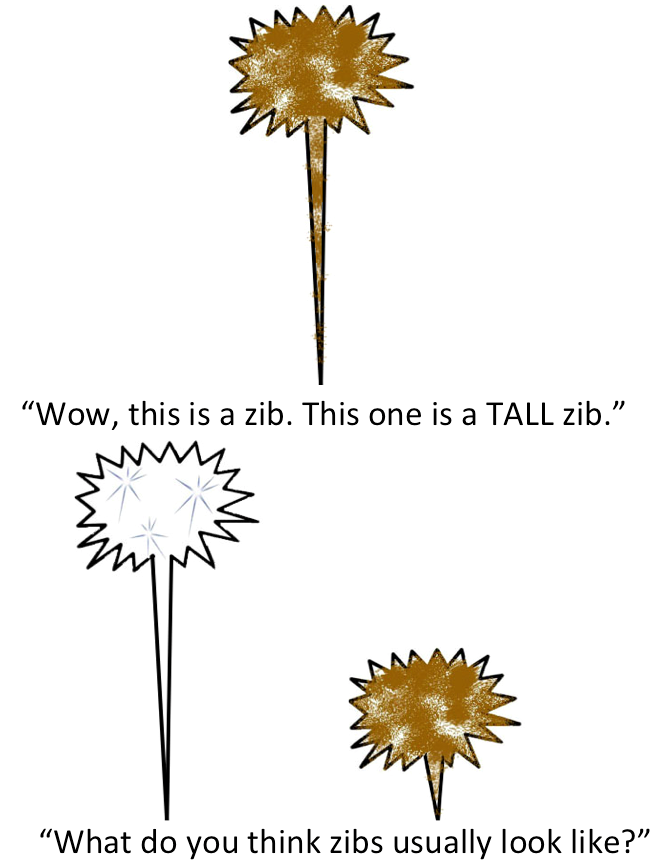
\includegraphics[width=3in]{figures/zib_example.png} 
    \caption{\label{fig:inanimate_demo} Example test trial. Participants were introduced to a base shape (top) described with either a feature or size adjective. They were then shown two images, one that differed from the exemplar by a feature contrast (e.g. dirty vs. clean, left) and one by a size contrast (e.g. tall vs. short, right), and were asked to point to which picture they thought was also a member of the same category. } 
  \end{center} 
\end{figure}	

We constructed the experiment as a storybook, illustrated with colorful clipart images. The book contained two training trials and four test trials. Each test trial consisted of a novel shape (induction example) along with a pair of generalization stimuli: one that differed from the induction example only by size (e.g. tall versus short), and one image that differed from the exemplar only by a feature contrast (e.g., dirty versus clean; see example in Figure \ref{fig:inanimate_demo}). Two of the four trials used size adjectives and two of the trials used feature adjectives.
% Training trials were similar but showed familiar items (e.g. chocolate milk as the induction example, with plain milk and orange juice as the generalization stimuli).  
Size terms were \emph{small} (vs. big), \emph{long} (vs. short), \emph{tall} (vs. short), and \emph{short} (vs. long);  feature contrasts were \emph{broken} (vs. unbroken), \emph{pointy} (vs. smooth), \emph{dirty} (vs. clean), and \emph{wet} (vs. dry).  To ensure that children were familiar with the words we used, we included a posttest of two-alternative displays.  Children were able to recognize all of the contrasts used in our task, with 90\% accuracy for 3--3.5 year-olds, 95\% for 3.5--4.0 year-olds, 96\% for 4.0--4.5 year-olds, and 98\% for 4.5--5.0 year-olds.  

\subsubsection{Procedure}

The experimenter read the storybook with children individually in a quiet room at their preschool or the CDM.  At the museum, parents accompanied children and sat next to or behind them.  If siblings were present, they were offered quiet activities such as coloring or reading.
%Siblings were sometimes also present, and were offered quiet activities such as coloring or reading. 

To begin the book, children were introduced to a character named Allen the Alien who was visiting planet Earth.  They then participated in two training trials containing familiar items to teach Allen about some things on Earth and get children used to the study design.  Training trials featured adjectives other than those used in test trials, and training pictures displayed only one relevant contrast choice.  For example, children were shown a picture of chocolate milk followed by two pictures, one of plain milk and one of orange juice. Children were told, ``This is a special kind of milk. This is \emph{chocolate} milk.  What does milk usually look like?  What does most milk look like?" and prompted to point to the picture.\footnote{Our test question is framed around prototypically in order to make the strongest case for inferring an implied dimension of contrast from adjective use: asking what something \emph{usually} looks like helps provide pragmatic support that the prenominal modifier is describing something atypical, and that other category members differ by that property. Although we expect children to comprehend \emph{most} and \emph{usually} at the ages tested \cite{halberda2008}, we help illustrate the relationship between adjective use and typically through familiar examples in the training trials.    }
%{The goals of the training trials were to 1) have children practice making selections by pointing, 2) remind them that adjectives point out variations, and 3) familiarize them with the framing of identifying what something \emph{usually} looks like. We ask about prototypically in order to make the clearest test case for inferring an implied dimension of contrast from adjective use.
 %1) remind children that adjectives point out variations, 2) familiarize them with the framing of identifying what something \emph{usually} looks like, and 3) have them practice making selections by pointing. We Our test question asks about prototypically in order to make the clearest test case for inferring contrast from adjective use: a prenominal modifier suggests that something is atypical along the referenced property dimension.}. 
On the rare occasion that children answered incorrectly, the experimenter repeated the statements and encouraged children until they answered correctly.  

After the training trials, children participated in four test trials.  For each test trial, children were shown a picture of an induction example and told something about it, e.g. ``This is a special kind of zib.  This is a tall zib.''  They were then shown two similar pictures, one that differed from the exemplar only by a feature (e.g., a tall clean zib) and one that differed from the exemplar only by size (e.g., a short dirty zib), and were asked ``What do you think zibs usually look like?  What do you think most zibs look like?'' They were prompted to select one of the non-exemplar images. 

Participants were assigned to one of two lists, counterbalanced for adjective type and picture order.  Adjectives were focused using contrastive stress. The experimenter averted her gaze while children pointed to their responses.  Responses were coded online and double-coded offline using a video recording of the testing session.  The task took about ten minutes to complete. 

The task was adapted to an online format for adult participants. They viewed a single trial composed of one of the picture triads and read the same text that was spoken to children. We used only a single trial for adults to avoid inducing task demands caused by repeating the same type of inference \cite{frank2012}. Picture type, side, and adjective were counterbalanced across participants.  Adults indicated their response using a radio button below their image selection.  Participants were paid 25 cents for completing the task, which took about two minutes to complete. 

\subsection{Results and discussion}

\begin{figure}[t] 
  \begin{center} 
    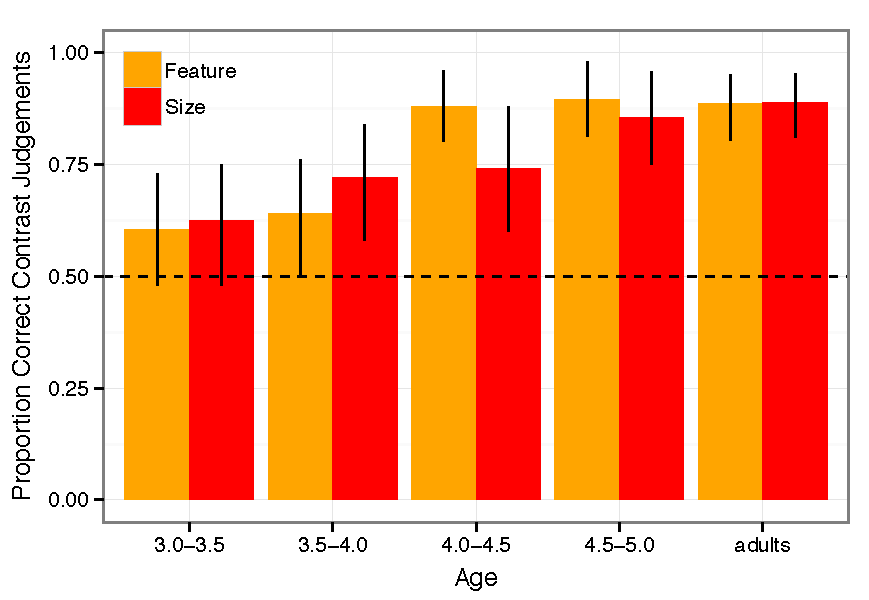
\includegraphics[width=5in]{figures/expt1_mod.pdf} 
    \caption{\label{fig:expt1_kidsAdults} Mean proportion correct contrast judgments for preschoolers and adults in Experiment 1. Yellow bars depict feature adjective trials and red bars depict size adjective trials. Dashed line represents chance; error bars show 95\% confidence intervals computed by non-parametric bootstrap.}
    %95\% confidence intervals.} 
  \end{center} 
  % \vspace{-2.0ex} 
\end{figure}	

Preschoolers' ability to make correct contrast inferences increased across the age range we tested (Figure \ref{fig:expt1_kidsAdults}).\footnote{Data and analysis code can be found at \url{http://github.com/ahorowit/aliens}.} We categorized a response as correct---representing what we will call a \emph{contrast inference}---if participants selected the item that differed from the exemplar along the referenced dimension (e.g., they chose the short item if the exemplar was referred as ``tall,'' and the clean item if it was described as ``dirty'').  The youngest children in our sample (age 3.0--3.5 years) were marginally above chance ($t(23) = 1.84$, $p = .08$) in their contrast inferences across adjective types, and all other age groups were above chance (all $p$s $< .01$). These results indicate that preschoolers are sensitive to adjectives as conveying contrast information about a relevant property dimension.


%The youngest children in our sample were numerically above chance in their responding across categories ($M=.61$) but were only marginally above chance, consolidating across adjective types ($t(23) = 1.84$, $p = .08$). All other groups were above chance (all $p$s $< .01$). 

To measure differences across adjective types and age groups, we used a logistic mixed effect model, predicting correct responses as the interaction of age and contrast type, with random intercept and slope (reflecting contrast type) for each participant.  Children made increasingly more correct contrast judgments with age ($\beta = 1.52$, $p < .0001$). There was no significant effect of contrast type (feature vs. size adjectives), and there was no interaction between age and contrast type, suggesting that participants across ages did not differ in their responses to different property types.  Overall, these analyses show that children demonstrate an increasing sensitivity to implicit contrast information from prenominal adjective use.  

% Rather than selecting the image that matched the named property, adults and children both selected the contrasting property.  


% Adults had no difficulty inferring contrast from adjective use in our task, and preschoolers showed a developmental increase in performance before reaching that of adults by age 5.  


\section{Experiment 2}

% In our first set of experiments, we found that adults consistently made contrast inferences from adjective use, while preschoolers gained sensitivity to how speakers mark relevant property information with age.  They may begin by appreciating that scalar opposites are paired, and that use of one term (e.g. \emph{wet}) implies contrast with its opposite (i.e. \emph{dry}). 

In Experiment 1, we provided a supportive scaffolding to help children recognize that adjectives were being used contrastively: We told them explicitly that ``This is a special kind of tibu.'' Even with the support of these cues, the inferences that we test are challenging: children must comprehend the modified noun phrase, recognize that it is being used contrastively, and then select the item that \emph{differs} from the property named rather than selecting the visual match. Despite these demands, preschoolers overall performed remarkably well on the task.  

In Experiment 2, we removed this contrastive framing to test whether the older children (who succeeded handily in Experiment 1) could still make contrast inferences based on the presence of a contrasting adjective alone, a far more subtle cue. Our revised framing was ``This is a tibu. This is a small tibu.'' We hypothesized that this \emph{adjective only} condition would make the contrast inference substantially more difficult. Previous work on pragmatic inference has suggested that one major problem for preschool children in making inferences about contrasting terms is summoning to mind alternative terms that could have been used (e.g. that ``some'' is a weaker alternative to ``all''; \citeNP{barner2011}). For this reason, we attempted to alleviate this burden in our task by providing children with pre-training on the relevant contrasts used at test. In this \emph{alternatives pre-exposure} condition, we read children a book highlighting the polar opposites prior to the experimental task to remind children that, for example, ``dirty'' is an alternative to ``clean.'' We predicted that the increased experience comparing adjective alternatives in this condition would help support children's ability to make contrast inferences at test.


\subsection{Methods}

\subsubsection{Participants}

A new sample of 96 children was recruited from Bing Nursery School.  Because of the presumed increased difficulty of this task, we recruited children from the older age groups: 4.0--4.5 years (n=48, mean age 4;4) and 4.5---5.0 years (n=48, mean age 4;9).  Half of the children in each age group (24 younger 4s and 24 older 4s) were randomly assigned to each of the conditions (\emph{Adjective Only} and \emph{Alternatives Pre-Exposure}). Four children were excluded for not completing all four trials of the task. 

We also ran a new group of 128 adult participants in the \emph{Adjective Only} condition on Amazon's Mechanical Turk.  All participants were reported to be US residents and native English speakers.  They were informed that the task was designed for children.  Seven were excluded for failing to complete the task. 

\subsubsection{Materials}

\begin{figure}[t] 
  \begin{center} 
    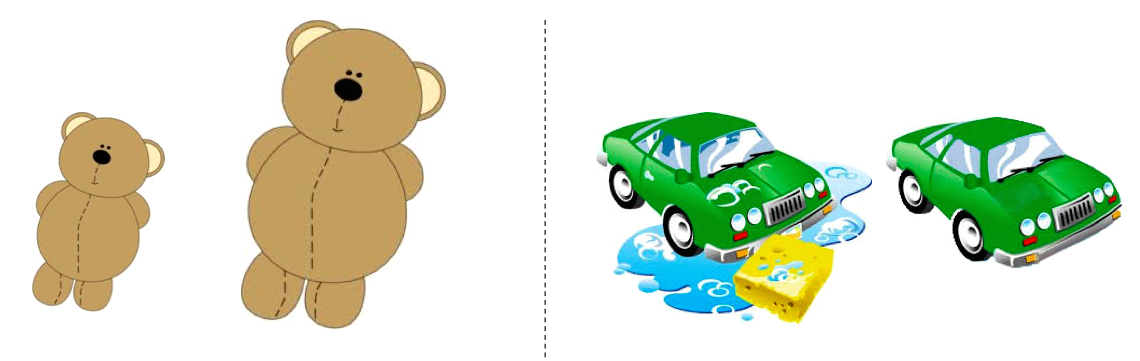
\includegraphics[width=4in]{figures/aliens_book_demo_mod.png} 
    \caption{\label{fig:book_demo} Sample images from the Alternatives Pre-Exposure book in Experiment 2. Left: example size contrast (small bear vs. big bear). Right: example feature contrast (wet car vs. dry car). }
  \end{center} 
\end{figure}

Stimuli were identical to Experiment 1. In the Alternatives Pre-Exposure condition, participants read a book prior to the testing procedure. The book consisted of clip art images of familiar items depicting the same size and feature contrasts terms portrayed in the test book. Opposites were paired so that scalar contrasts were viewed simultaneously and stated consecutively (e.g. ``Here is a small teddy bear. Here is a big teddy bear.'').  Sample images are presented in Figure \ref{fig:book_demo}.


\subsubsection{Procedure}

Procedures for the experimental task were identical to Experiment 1 with the exception that the referential phrase was minimized by removing the phrase ``special kind of'' to reduce contrast cues other than the adjective.  Instead, participants heard only ``This is a [zib]. This is a [tall zib].''  Children in the Alternatives Pre-Exposure condition were told that they would be reading two books in the experimental session. The experimenter read the adjectives book with children, labeling each picture in a neutral way on each page before reading the test book. Contrastive stress was emphasized for all adjectives in the Pre-Exposure book and in the test trials for both conditions. As in Experiment 1, adult participants were randomly assigned to a single test trial presented online.  

\subsection{Results and discussion}

\begin{figure}[t] 
  \begin{center} 
    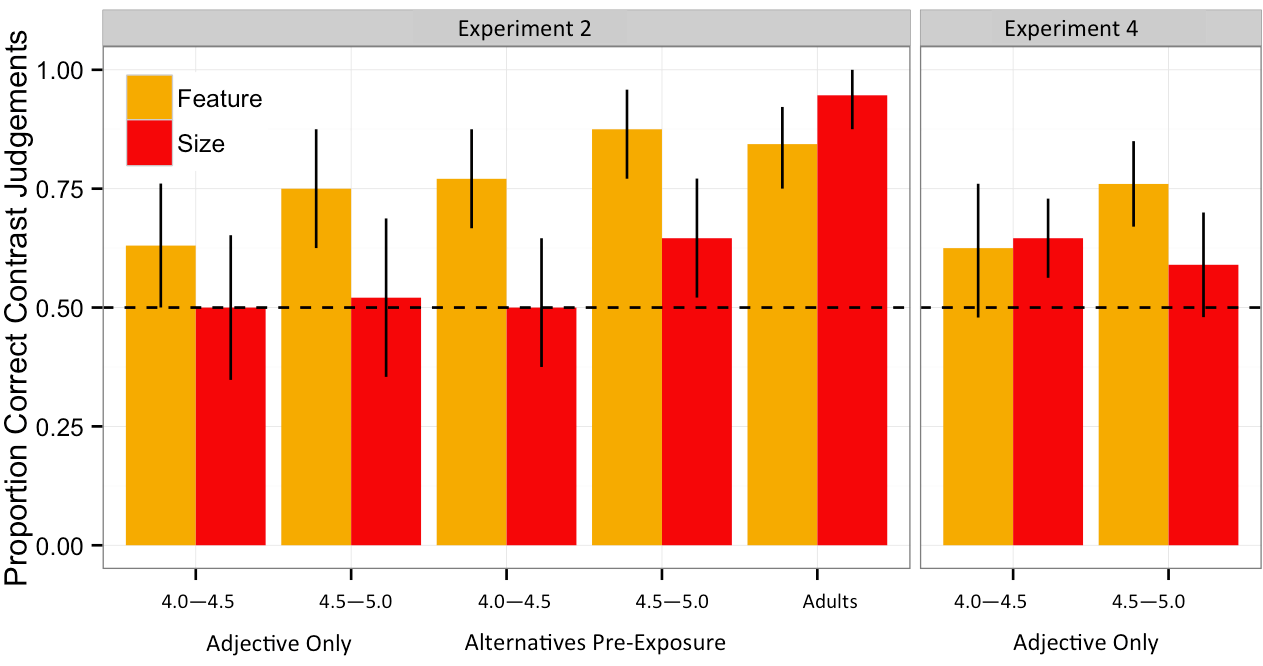
\includegraphics[width=6in]{figures/expts2And4.png} 
    \caption{\label{fig:expt2_kidsAdults} Preschoolers' and adults' proportion correct performance for the \emph{Adjective Only} and \emph{Alternatives Pre-Exposure} conditions in Experiment 2. Adults did not see the pre-exposure trials. Dashed line shows chance performance; error bars show 95\% confidence intervals.}
  \end{center} 
  % \vspace{-2.0ex} 
\end{figure}

With the removal of supportive language indicating contrast, performance in Experiment 2 was substantially lower than in Experiment 1. Contrast selections in size trials were especially low, while contrast judgements in feature trials remained higher. In the Adjective Only condition, averaging across adjective types, 4.0-year-olds were not above chance ($t(22) = 1.10$, $p = .28$), but 4.5-year-olds were ($t(23)=2.18$, $p = .04$). Breaking performance down by adjective type, on feature trials the younger 4s were marginally above chance, while the older 4s were substantially above chance ($t(22) = 1.82$, $p = .08$ and $t(23)=3.71$, $p = .001$). Both groups' performance did not differ from chance for size adjectives. Thus, without the contrastive language in Experiment 1, children had a substantially harder time but the oldest children could still make contrast inferences at above-chance levels for feature adjectives. 

One potential source of the asymmetry between feature and size adjectives could be due to the relatively greater contrast implied by our featural adjectives. Saying that something is ``dirty'' almost always implies a changed state from having been clean at another point in time. In contrast, saying something is ``tall'' can imply that there are shorter others---but it can also simply reflect some sort of general, stable comment on height. If this ambiguity about the contrastiveness of the size adjectives was the source of the lowered performance in the Adjective Only condition, the Alternatives Pre-Exposure condition might increase performance for size adjectives by virtue of highlighting the contrastive use of alternative size terms. 

Congruent with this hypothesis, the alternatives pre-exposure appeared to boost performance somewhat. Children in the Alternatives Pre-Exposure condition were above chance at both ages ($t(23) = 2.33$, $p = .03$ and $t(23) = 6.33$, $p < .0001$), aggregating across adjective types. Breaking down by adjective types, the younger 4s were above chance for feature but not size adjectives ($t(23) = 4.51$, $p = .0001$ and $t(23)=0$, $p = 1$). Older children were above chance on both ($t(23) = 8.31$, $p < .0001$ and $t(23)= 2.07$, $p = .05$). Nevertheless, no pairwise tests between the Adjective Only and Alternatives Pre-Exposure conditions reached significance. 

We again analyzed our results using a logistic mixed model. We initially fit a model that included all interactions of age, adjective type, and book type but found that no effects reached significance; indeed, this model did not increase fit over a model that only included main effects ($\chi^2(4) = 2.47$, $p = .65$). This main-effects only model included a significant effect of adjective type such that they made fewer contrast selections on size trials than feature trials ($\beta = -1.08$, $p < .0001$). It also included marginal effects of age and book type ($\beta = 1.04$, $p = .07$ and $\beta = .50$, $p = .09$, respectively), indicating that older children performed better than younger children, and that performance was higher in the Alternatives Pre-Exposure condition than the Adjectives Only condition. 


%included a significant negative coefficient on size adjectives ($\beta = -1.08$, $p < .0001$) and marginal effects of age and book type ($\beta = 1.04$, $p = .07$ and $\beta = .50$, $p = .09$, respectively). 

In sum, Experiment 2 provides support for the hypothesis that children's judgments in Experiment 1 were strengthened by the presence of the contrastive language ``a special kind of.'' When we removed this language, performance dropped markedly, especially for size adjectives (which might not be as clearly contrastive as feature adjectives). We also saw some signs that pre-exposure to a storybook that used the target adjectives contrastively improved performance, providing additional support to the idea that it was specifically the recognition of pragmatic contrasts that led children to make the appropriate generalization. 

One possible alternative explanation for our findings is that contrast inferences were in fact not warranted by the simpler adjective framing (rather than being warranted but not being identified by children). Ruling out this explanation, the performance of adults in Experiment 2 (without supportive language) was essentially identical to that of adults in Experiment 1. Thus, we believe that the contrastive framing in Experiment 1 helped children differentially in interpreting the contrast inference implied by the use of the adjective features. It appears that children can recognize that prenominal adjectives imply 

\section{Experiment 3} 

In Experiment 3, we tested the extent of children's inferences from contrastive adjective use by examining their performance in a free-response task. One possibility in Experiments 1 and 2 was that children in fact did not infer contrast immediately from the linguistic frame and adjective, but instead recognized that the two-alternative forced choice task required a contrastive interpretation of the adjective. A free response task circumvents this issue by testing children's interpretation of the concept without asking them to choose between alternatives. For the linguistic framing in this experiment, we chose an intermediate level of support for contrast; less extreme than Experiment 1 but more supportive than Experiment 2: we told children that ``This is a plizzle. There are different kinds of plizzles. This one is a small plizzle.'' 

\subsection{Methods}

\subsubsection{Participants}

We recruited a new planned sample of 24 4-year-old children (mean age 4;6) from the CDM.  Only children whose parents reported that they heard English at least 75\% of the time were included in the final sample.  Two participants were excluded for using less than this amount of English, and one participant was excluded for not producing responses to the experimenter's questions.

\subsubsection{Materials}

We used a similar task design as Experiments 1 and 2, but showed children only a single picture rather than a triad.  In addition, because some of the original items depicted contrasts in which one pole was visually salient but perhaps difficult for children to name (e.g. ``broken'' vs. ``unbroken''), we modified the set of items we used.  The named size contrasts used were \emph{small} (vs. big), \emph{tall} (vs. short), \emph{long} (vs. short), and \emph{skinny} (vs. fat).  The named feature contrasts were \emph{hot} (vs. cold), \emph{dark} (vs. light), \emph{wet} (vs. dry), and \emph{open} (vs. closed).  We also included a post-test to ensure that children were familiar with all of the properties used in the task.  Children successfully identified pictures that corresponded with the meanings of the adjectives in 96\% of trials.

\subsubsection{Procedure}

The experimenter read the storybook with children individually in a quiet room at the CDM. As before, children were introduced to Allen the Alien and then participated in two training trials with familiar items. Unlike in  Experiments 1 and 2, children saw only a single image per trial. For example, in a training trial, children were shown a picture of a heart-shaped cookie and told, ``This is a cookie.  There are different kinds of cookies.  This one is a heart-shaped cookie.  What do other cookies look like?'' Most children answered immediately that most cookies are \emph{round} or \emph{circle}-shaped. A few children were slower to respond, and were promoted to think again what most cookies look like. If they still did not respond, they were asked what shape most cookies are.  If children provided an answer other than shape, they were encouraged to think about the description again (e.g. ``You're right, cookies can be different flavors. Did you see this one is heart-shaped?  What do most cookies look like?''). 

Following the two training trials, children participated in four test trials.  For each test trial, children were shown a picture of a single exemplar and told something about it, e.g. ``Wow, this is a plizzle. There are different kinds of plizzles. This one is a small plizzle.  What do you think other plizzles look like?'' Their verbal responses were recorded.  Two of the test trials referred to size adjectives (e.g. \emph{small}), and two of the trials referred to feature adjectives (e.g. \emph{hot}).  The order of trial items varied across two lists, each of which was counterbalanced for adjective type and picture order.  Adjectives were focused using contrastive stress. Responses were coded online and double-coded offline using a video recording of the testing session.  The task took about ten minutes to complete. 

\subsection{Results and discussion}

\begin{figure}[t] 
  \begin{center} 
    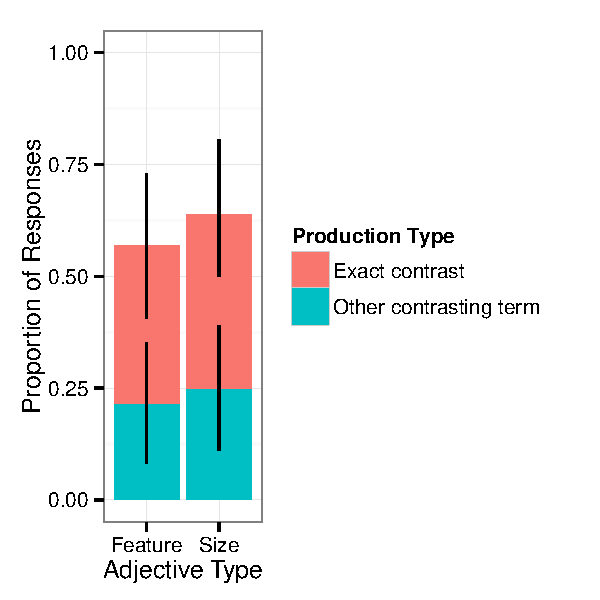
\includegraphics[width=3.5in]{figures/expt3.pdf} 
    \caption{\label{fig:freeResponse} Four-year-olds' free response descriptions of other category members upon hearing a feature adjective (left) or size adjective (right).  Productions were coded as being \emph{Exact contrasts} if they were opposite the description and as being \emph{Other contrasting terms} if they were related to the referenced property but neither a direct contrast nor an exact match. Error bars show 95\% confidence intervals. }
  \end{center} 
\end{figure}

Despite the open-ended nature of the task, children gave contrastive responses more than half of the time (57\% and 64\% overall for feature and size, Figure \ref{fig:freeResponse}).  We coded responses as either an \emph{Exact contrast} (e.g. hearing ``small'' and saying ``big'') or as an \emph{Other contrasting term} if they were an approximate contrast to the named property (e.g. hearing ``small'' and saying a size property other than ``big'', e.g. ``tall''). Matching, non-contrastive descriptions (e.g. hearing ``small'' and repeating ``small'') were not included in the approximate contrast group. More than a third of productions were exact opposites (35\% for feature terms and 39\% for size terms), and another quarter were non-exact contrasts but related to the stated property information (22\% for feature terms and 25\% for size terms). There were no differences in the proportion of response scores across feature and size trials. Thus, Experiment 3 provides evidence that, even without seeing a contrastive alternative test item, children were able to spontaneously generate appropriate descriptions based on the adjective the speaker used. These results suggest that children can consider possible contrastive implications from word choice cues, and the presence of the visual alternatives in the previous experiments may have even dampened their performance. Our minimal design with two related visual alternatives (a property match and a property contrast) may have made it more cognitively taxing for children for children to hold their inferences in mind and inhibit selecting the named property than merely generating likely contexts on their own.

\section{Experiment 4} 

Experiments 1--3 show that preschoolers can spontaneously infer a property dimension of contrast from the presence of an adjective. We wondered, however, how much children's performance was an artifact of the particular modifier terms used, which tended to convey marked, atypical properties For example, children may hear ``dirty'' and select that other category members tend to be clean based on their baseline assumptions that \emph{clean} is the default, regardless of the adjective used. Thus in Experiment 4, we ran another version of the experiment that fully counterbalanced adjective references across both ends of the opposite scales (i.e. instead of pitting a single feature vs. size term---``dirty'' vs. ``tall''---we also included references to their opposites---``clean'' vs. ``short'').  Children's patterns of responses remained the same in their version of the experiment, suggesting that their performance is reflecting sensitivity to pragmatic implications of word choice generally rather than base rate assumptions about property states.


\subsection{Methods}

\subsubsection{Participants}

We recruited a new planned sample of 48 children into two age groups: 4.0--4.5 years (n=24, mean age 4;3), and 4.5--5.0 years (n=24, mean age 4;8).  Half of the sample of each age group was recruited from the Bing Nursery School and half was recruited from the the CDM.

\subsubsection{Materials}

Stimuli were combined and mostly identical to the previous experiments, with some modifications to depict unique, namable feature opposites across 8 test trials. Four size properties (\emph{big---small, tall---short, fat---skinny, long---short}) were repeated twice so that each term was represented as an exemplar once per participant.  Each test trial featured a unique feature contrast: \emph{dirty---clean, wet---dry, pointy---round, hot---cold. dark---bright, open---closed, soft---hard,} and \emph{full---empty}.  

\subsubsection{Procedure}

The procedure was identical to the Adjectives Only condition in Experiment 2. Children participated in 8 trials, counterbalanced by order (forward or reverse, adjective type (feature vs. size), opposite term (e.g. ``dirty,'' ``clean,'' ``tall,'' or ``short''), and target location. All adjectives were focused using contrastive stress. 

\subsection{Results and discussion}

Four-year-olds made contrast inferences for all adjective references in the task, regardless of the property type (size or feature term) and polarity (which end of the opposite scale). These findings indicate that preschoolers are sensitive to adjective use generally, regardless of the typicality; they were equally likely to make contrast selections for ``dirty'' implying that others are clean as for ``clean'' implying that others are dirty even without the cue of contrastive framing (i.e. without reference to the exemplar being ``special'').

Overall, younger and older 4s selected the property contrast reliably above chance ($t(23) = 3.05$, $p<.01$ and $t(24) = 3.99$, $p<.001$, respectively). Examining performance by age group and trial type more closely, younger 4s made contrast selections reliably above chance in size trials ($t(23)=3.44$, $p<.01$) and marginally above chance for feature trials ($t(23)=1.73$, $p=0.09$). Older 4s showed a slightly different pattern, selecting the contrast reliably on feature trials ($t(24)=5.32$, $p<.0001$) but at chance for size trials ($t(24)=1.56$, $p=.13$). To examine children's pattern of responses more closely, we ran a logistic mixed effect model predicting correct responses as an interaction of contrast type and age, with random slope (reflecting contrast type) for each participant.  A marginal effect of adjective type emerged, such that children made more contrast selections for size than feature trials overall ($\beta = 7.69$, $p = .09$). There was also a marginally significant interaction between trial type and age, such indicating that contrast selections for size trials decreased with age ($\beta = -1.85$, $p = .08$).  Despite these marginal variabilities, overall we see that 4-year-olds make contrast inferences from adjective use across a range of properties types. 


\section{General Discussion}

If a speaker describes an ``art museum,'' can children learn that there are other types of museums? And if children hear someone described as a ``female scientist'' or ``male librarian,'' will they make (potentially harmful) inferences about gender-typical roles? Our findings support the idea that children are indeed sensitive to contrasts of this type. In our experiments, they were able to learn from not just the literal content of a speaker's utterance, but from the choices she made in expressing that content; and they did so most effectively in cases where the particular contrast of interest was made salient.

In Experiment 1, preschoolers reliably made contrast inferences from size and feature adjectives with the support of a contrastive linguistic framing.  In Experiment 2, we found that unlike adults, 4-year-olds had difficulty making these inferences when the supportive framing was removed. Their performance increased somewhat after exposure to the relevant adjective contrasts, however, suggesting that a number of cues to the contrastiveness of a particular adjective could contribute to their ability to make inferences. Finally, in Experiment 3, which used a free-response task, four-year-olds were able to generate the relevant property contrasts (without seeing them pictured in the two-alternative-forced choice we used in the other experiments). Taken together, our results suggest that preschoolers can reason about speakers' adjective choices as providing information not only about the particular entity being described at the time, but also about other category members. 

Although the design of our task was simple, it nevertheless required a counterintuitive response: hearing a description and inferring that its opposite was represented in the broader set. In other words, children needed to process the stated adjective and then select the picture that \emph{differed} from that description instead of the one that shared that property, even though both picture options were available. The task thus involved both pragmatic reasoning about how people use language, and also the exercise of executive function in inhibiting the bias to  match the description directly at test.  We found that preschoolers nonetheless made contrast inferences, though performance was stronger in older children; the development of executive function in this age range provides a plausible source for the developmental effects we observed \cite{davidson2006,zelazo2003}. 

Our data speak to children's ability to learn one particular piece of information from pragmatic language use: the typical property for exemplars of a category. We selected this particular example because the generalization of category structure from individual exemplars is a key problem for children \cite{markman1991}. But there are potentially many different inferences that could be made on the basis of the same sort of optional modification. As in the case of ``art museum,'' sometimes a contrastive modifier does not license specific inferences about what is typical of a category (i.e. if ``art'' does not have an opposite, what can we infer about other museums?) but only that there is some important variability in a particular dimension (there are other types of museums other than art museums). The pragmatic and discourse context of an utterance can also affect the kind of inference that is licensed by a contrastive modifier: Depending on context, labeling someone as a ``good student'' can imply that others in the comparison set are either better (where the student is implied to be ``merely good'') or worse (where the student is ``very good''). Future work should investigate a broader range of cases of pragmatic learning, from other kinds of world knowledge to the idiosyncrasies of social judgement that are implied by descriptive language. 

Our experiments contribute to the growing literature suggesting that children consider how and why evidence is generated to reason about the social world, in both non-linguistic and linguistic contexts. As reviewed above, even young children robustly infer probabilities from random sampling while making inferences about social preferences or generalizable knowledge from conspicuous non-random sampling \cite{xu2009, kushnir2010, butler2012}. In the domain of language, preschoolers are beginning to make similar (pragmatic) inferences about the motivations for language use \cite<e.g.>{stiller2014,katsos2011}, though many factors may constrain their ability to succeed in more complex situations \cite{papafragou2003,barner2011}. 

The \emph{alternatives hypothesis}---that children's ability to make inferences is often constrained by their ability to bring to mind and contrast the relevant inferential alternatives---has been proposed to explain children's failures in pragmatic reasoning \cite{chierchia2001,barner2011}. In the case of scalar implicature, these alternatives can be quantifiers like ``some'' and ``all''; in our case, they were pairs of polar adjectives. In both cases, the pragmatic inference is supported by an appreciation of what \emph{wasn't} said. Our pre-exposure manipulation in Experiment 2 provides some preliminary evidence that the alternatives hypothesis explains children's difficulty in our task. An earlier study we conducted with color adjectives also supports this hypothesis \cite{horowitz2012}. Four-year-olds in this study were considerably more proficient in making contrast inferences with size terms than with colors. One explanation for the difficulty that children had with colors was the lack of an obvious alternative: While a ``\emph{small} tibu'' might be exceptional relative to the larger, more typical tibus, a ``\emph{blue} tibu'' less clearly implies what color other tibus are (other than not being blue). Although the stimuli in this earlier experiment were different than those used in the current study and hence direct numerical comparisons between levels of performance are not possible, it nevertheless provides additional circumstantial evidence about the role of pragmatic alternatives in allowing such inferences. 

Most work investigating children's pragmatic abilities has focused on reasoning about speakers' intended meanings. In contrast, we examined children's inferences about the state of the world that would lead a speaker to make particular production choices. While preschoolers show evidence of learning generalizable knowledge from specific descriptions based on framing cues \cite{cimpian2009}, our work suggests an additional pragmatic route to such general knowledge. In this way, we connect the mechanisms of pragmatic inference with processes of social learning and generalization. If children assume that speakers are communicating pragmatically, then they can take advantage of opportunities for learning wherever they recognize a speaker's choice to produce an utterance in one form over another. 

\bibliographystyle{apacite2}
\bibliography{ADJ2}

\end{document}
